\documentclass[a4paper, 11pt,titlepage, openright, twoside]{report}
\usepackage[utf8]{inputenc}
\usepackage[T1]{fontenc}
\usepackage{silence}
\usepackage{amsmath,amsfonts,amssymb,amsthm}
\usepackage{mathtools}
\usepackage[inline]{enumitem}
\usepackage{newunicodechar}
\usepackage[margin=3cm,bindingoffset=1cm]{geometry}
\usepackage{stmaryrd}
\SetSymbolFont{stmry}{bold}{U}{stmry}{m}{n}
% https://tex.stackexchange.com/a/106719
\DeclareSymbolFont{sfletters}{OML}{cmbrm}{m}{it}
\usepackage[nopatch=footnote]{microtype}
\usepackage[dvipsnames]{xcolor}
\usepackage{mathpartir}
\usepackage{biblatex}
\usepackage{hyperref}
\usepackage{cleveref}
\usepackage{tikz}
\usepackage{tikz-cd}
\usepackage{listings}
\lstset{basicstyle= \footnotesize \ttfamily}
\lstset{language=ml}

\usepackage[nodisplayskipstretch]{setspace}
\setlength{\parskip}{0pt}

\addbibresource{refs.bib}


\title{\textbf{A Fine Calculus for Static Delimited Control}}
\author{Wiktor Kuchta}

\date{60 września 2024} %TODO

\usepackage{titling}

\renewcommand \maketitlehookb {
  \begin{center}\large
  Fajny rachunek dla statycznie ograniczonych operatorów sterowania
  \end{center}
  \vfil
}

\renewcommand \maketitlehookc {
  \vfil
  \begin{center}
  \large Praca magisterska \\[0.85em]
  \begin{tabular}[t]{rl}
  \textbf{Promotor:} & dr hab. Dariusz Biernacki
  \end{tabular}\end{center}
  \vfil\vfil\vfil\vfil
  \begin{center}Uniwersytet Wroc\l{}awski\\
  Wydzia\l{} Matematyki i Informatyki\\
  Instytut Informatyki
  \end{center}
}


\newcommand{\shiftz}{\textsf{shift0}}
\newcommand{\abort}{\textsf{abort}}
\newcommand{\keyword}[1]{\textsf{\textup{#1}}}
\newcommand{\KwOp}{\keyword{op}}
\newcommand{\Op}{\KwOp\,}
\newcommand{\KwHandle}{\keyword{handle}}
\newcommand{\Handle}{\KwHandle\;}
\newcommand{\KwWith}{\keyword{with}}
\newcommand{\With}{\;\KwWith\;}
\newcommand{\KwRaise}{\keyword{raise}}
\newcommand{\Raise}{\KwRaise\;}
\newcommand{\Ask}{\textsf{ask}}
\newcommand{\KwTry}{\keyword{try}}
\newcommand{\Try}{\KwTry\;}
\newcommand{\KwLet}{\keyword{let}}
\newcommand{\Let}[3]{\keyword{let}\;#1\;\keyword{=}\;#2\;\keyword{in}\;#3}
\newcommand{\RLet}[3]{\Let{#1}{\raisebox{0.5 ex}{$#2$}}{#3}}
\newcommand{\KwLift}{\keyword{lift}}
\newcommand{\Lift}[1]{\KwLift\;#1}
\newcommand{\subst}[2]{\{#1{:=}#2\}}
\newcommand{\E}{\mathcal{E}}
\newcommand{\K}{\mathcal{K}}
\renewcommand{\S}{\mathcal{S}}
\newcommand{\A}{\mathcal{A}}
\newcommand{\kT}{\mathsf{T}}
\newcommand{\kE}{\mathsf{E}}
\newcommand{\kR}{\mathsf{R}}
\newcommand{\Free}{\textrm{-}\mathrm{free}}
\newcommand{\Obs}{\mathrm{Obs}}
\newcommand{\N}{\mathbb{N}}
\DeclareMathOperator{\dom}{dom}
\newcommand{\+}{\enspace}
\newcommand{\lStr}{\textsf{Str}}
\newcommand{\lPar}{\textsf{Par}}

\newtheorem{corollary}{Corollary}
\newtheorem{lemma}{Lemma}
\newtheorem{theorem}{Theorem}
\newtheorem{prop}{Proposition}


\newunicodechar{│}{\mid} % Digr vv
\newunicodechar{╱}{\mathbin{/}} % Digr FD
\newunicodechar{∷}{::} % Digr ::
\newunicodechar{□}{\square} % Digr OS
\newunicodechar{∅}{\emptyset} % Digr /0
\newunicodechar{α}{\alpha}
\newunicodechar{β}{\beta}
\newunicodechar{δ}{\delta} % Digr d*
\newunicodechar{ε}{\varepsilon}
\newunicodechar{γ}{\gamma} % Digr g*
\newunicodechar{ι}{\iota} % Digr i*
\newunicodechar{κ}{\kappa}
\newunicodechar{λ}{\lambda}
\newunicodechar{μ}{\mu}
\newunicodechar{ν}{\nu}
\newunicodechar{ρ}{\rho}
\newunicodechar{σ}{\sigma}
\newunicodechar{τ}{\tau}
\newunicodechar{η}{\eta} % Digr y*
\newunicodechar{Δ}{\Delta}
\newunicodechar{Γ}{\Gamma}
\newunicodechar{Ω}{\Omega} % digr W*
\newunicodechar{ℕ}{\N} % Digr NN 8469 nonstandard
\newunicodechar{⊆}{\subseteq} % Digr (_
\newunicodechar{∪}{\cup} % Digr )U
\newunicodechar{∈}{\in} % Digr (-
\newunicodechar{∃}{\exists} % Digr TE
\newunicodechar{∀}{\forall} % Digr FA
\newunicodechar{∧}{\wedge} % Digr AN
\newunicodechar{∨}{\vee} % Digr OR
\newunicodechar{⊥}{\bot} % Digr -T
\newunicodechar{⊢}{\vdash} % Digr \- 8866 nonstandard
\newunicodechar{⊨}{\models} % Digr \= 8872 nonstandard
\newunicodechar{⊤}{\top} % Digr TO 8868 nonstandard
\newunicodechar{⇒}{\implies} % Digr =>
\newunicodechar{⇔}{\iff} % Digr ==
\newunicodechar{↦}{\mapsto} % Digr T> 8614 nonstandard
\newunicodechar{≠}{\neq}
\newunicodechar{⟦}{\llbracket} % Digr [[ 10214 nonstandard (needs pkg stmaryrd)
\newunicodechar{⟧}{\rrbracket} % Digr ]] 10215 nonstandard
\newunicodechar{≥}{\ge}
\newunicodechar{≤}{\le}
\newunicodechar{≡}{\equiv}
\newunicodechar{≈}{\approx}


% cursed
\WarningFilter{newunicodechar}{Redefining Unicode}
\newunicodechar{·}{\ifmmode\cdot\else\textperiodcentered\fi} % Digr .M
\newunicodechar{×}{\ifmmode\times\else\texttimes\fi} % Digr *X
\newunicodechar{→}{\ifmmode\rightarrow\else\textrightarrow\fi} % Digr ->
\newunicodechar{←}{\ifmmode\leftarrow\else\textleftarrow\fi} % Digr <-
\newunicodechar{…}{\ifmmode\dots\else\textellipsis\fi} % Digr .,
\newunicodechar{⟨}{\langle}
\newunicodechar{⟩}{\rangle}

\begin{document}

\maketitle


\thispagestyle{empty}
\cleardoublepage
\begin{abstract}
	We consider a variant of the call-by-value $λμ$-calculus extended with control delimiters,
	in which $μ$ becomes the static delimited control operator shift0.
	We propose new reduction rules for cases where the captured continuation can be determined statically.
	We prove the calculus confluent and adequate wrt.\,operational semantics.
	We then let delimiters carry data (resulting in a form of dynamic binding), which lets us express deep effect handlers.
	The new reductions cooperate with the encoding to let us statically handle effects.
	We also propose natural encodings of return clauses for delimiters.
%	We propose purity assertions for lightweight purity-based reasoning.
%	We prove the reduction is confluent and adequate wrt.\ operational semantics.
	We argue that the calculus is stronger than previous results in the literature and could form basis for
	reasoning and optimizations for the aforementioned forms of control.
	\begin{center} \rule[3pt]{300pt}{1pt} \end{center}
	polski
\end{abstract}


\thispagestyle{empty}
\cleardoublepage
\setcounter{page}{5}
\tableofcontents


\chapter{Introduction}
Consider a program of the following form in a language with (unnamed) exceptions:
\begin{align*}
	&\Try \\
	&\quad \Let{x}{e}{\Raise (x*2)} \\
	&\KwWith\; z.\,z*3
\end{align*}
If the execution gets to $\Raise (x*2)$, the handler will catch the exception and produce the result $x*2*3$.
%$$\Try \Let{x}{e}{\Raise (2*x)} \With z.\,3 * z$$
%We know that \textit{the} $\KwRaise$ (if we get to it) is going to be handled by \textit{the} handler.
%And in that case, $x*2$ is going to be multiplied by $3$.
How to \textit{optimize} the program, so that we only perform one multiplication, $x*6$?

We can ask a similar question for \textit{effect handlers}.
This generalization allows us to capture the \textit{continuation} of the \textit{operation} (a.k.a.\,\textit{generic effect}) we are handling
and bind it as a variable.
The conventional evaluation step rule is
$$\Handle E[\Op v] \With x\;k.\,e ↦  e\subst{x}{v}\subst{k}{λy.\,\Handle E[y] \With x\;k.\,e} $$
This is a form of \textit{static delimited control}: control because we capture continuations,
delimited because the continuation is delimited by the handler, and static because the delimiter remains
in the captured continuation.
%The last part is crucial.

Let's consider a similar example:
$$ \Handle \Let{x}{e}{\Op (x*2)} \With z\;k.\,k\,(z*3) $$
Similarly to the example of exceptions, we know that $\Op (x*2)$ will be handled
by the $z\;k.\,k\,(z*3)$ handler -- even if continuation capture occurs during the execution of $e$,
the $\KwOp$ and the $\KwHandle$ will stay together.

We therefore know the substitution that will be performed during the handling of the operation:
$z:=x*2$. Exactly this substitution is needed to rewrite the two multiplications into one.
We also can deduce the substitution $k:=λy.\,\Handle y \With z\;k.\,k\,(z*3)$.
But where to substitute? Certainly not in the handler's clause, because the clause is shared for all operations inside,
and $x$ is not even in scope.

Since we know the clause that will run for the specific operation,
instead of performing it, we can \textit{abort} the handler and execute the clause specialized with the specific substitutions.
That is, rewrite the $\Op (z*2)$ into
$$\A\,(k\,(z*3))\subst{z}{x*2}\subst{k}{λy.\,\Handle y \With z\;k.\,k\,(z*3)},$$
where $\A$ is the new \textit{abort} expression former.
We get
$$\Handle \Let{x}{e}{\A\,\big((λy.\,\Handle y \With z\;k.\,k\,(z*3)) (x*2*3)\big)} \With z\;k.\,k\,(z*3)$$
which simplifies to
$$\Handle \Let{x}{e}{\A\,(x*6)} \With z\;k.\,k\,(z*3)$$

Of course, this poses questions such as ``where does the abort come from?''.
One can also imagine that the general rewrite rule for this would be rather complicated...

The issue with conventional syntax for operations and effect handlers is that
the operations are \textit{passive}.
In a real implementation, when we get to an operation, we immediately begin the search for a handler.
The syntax does not reflect that, it doesn't say what happens next. It's just an operation name and a payload value.

We will therefore base our calculus for optimizations on the other static delimited control operator:
$\shiftz$. The conventional rule for $\shiftz$ and its delimiter \textsf{reset} (written $⟨·⟩$) is:
$$⟨E[\shiftz\,k.\,e]⟩ ↦ e\subst{k}{λy.\,⟨E[y]⟩}$$
Here, the $\shiftz$ assumes the active role by initiating capture of continuation $k$ and carrying the expression $e$ that says what to do with it,
while the delimiter is passive -- it merely delimits.
We can now express \textsf{abort} simply as a $\shiftz$ that ignores the continuation: $\textsf{abort}\,e ≡ \shiftz\,\_.\,e$.

To express effect handlers, we will extend delimiters by letting them carry a value.
The value will be a lambda abstraction $λz\;k.\,e$ representing the handler's clause.
An operation will be a $\shiftz$ that explicitly asks for it and applies the payload and continuation.

Finally, to achieve fine-grained steps instead of complex rules that move entire contexts around,
we will get rid of the irregularity that is the $λ$-abstraction wrapping the continuation.
Delimited continuations will not be represented as call-by-value functions, but instead
as their own sort with the ability to plug in any expression, not just a value.
This lets us use structural substitution known from the $λμ$-calculus and all the benefits it brings \cite{benefit}.

\chapter{Syntax}

\begin{figure}
\begin{align*}
	\text{values} &&v,u &::= x │ λx.\,e \\
	\text{expressions} &&e,t &::= v │ v\;v │ \Let{x}{e}{t} │ \S κ.\,e │ ⟨e / v⟩ │ κ[e] │ \Ask(κ) \\
	\text{evaluation contexts}&&E   &::= □ │ \Let{x}{E}{t} \\
	\text{metacontinuations}&&K   &::= □ │ \Let{x}{K}{t} │ κ[K] │ ⟨K/v⟩
\end{align*}
\caption{Syntax.}
\label{syntax}
\end{figure}

The syntax of the calculus is in figure \ref{syntax}.
We base it on a fine-grained call-by-value $λ$-calculus,
meaning that the subterms of application $v\;u$ are values
and computations have to be sequenced with $\KwLet$.
We use the notation $\S κ.\,e$ for the generalization of $\shiftz$ to continuation parameters.
It is analogous to the $μ$ operator from the $λμ$-calculus.
We will use the shorthand $\A\,e ≡ \S\_.\,e$ for an abort, i.e. an $\S$ that ignores the captured continuation.
The construct $⟨e/v⟩$ delimits continuations captured in $e$ and carries a value $v$.
We use the notation $κ[e]$ for plugging the expression $e$ into a continuation $κ$.
The $λμ$-calculus conventionally uses the notation $[κ]e$, but we abandon it
as it's inconsistent with the metanotation of plugging an expression into a context.
The value $\Ask (κ)$ refers to the value carried by the delimiter which delimited $κ$.

Contexts are terms with a hole ($□$), with $C[e]$ denoting substituting (or plugging)
the expression $e$ for the hole in $C$. We can also plug a context into a context, as in $C[C']$,
to form another context.

The operational semantics are in figure \ref{step}.
The last two rules make use of substitution for continuation variables.
We extend the notion of structural substitution of the $λμ$-calculus to the new $\Ask(κ)$ construct.

Formally, we can consider \textit{preterms}, where we generalize $κ[e]$ and $\Ask(κ)$ into $K[e]$ and $\Ask(K)$.
There, the substitution for continuation variables is defined in the natural way:
$κ[K]\subst{κ}{K'} ≡ K'[K\subst{κ}{K'}]$.

Now, we normalize preterms into terms according to the following rules:
\begin{align*}
	(□)[e] &→ e \\
	(\Let{x}{K}{t})[e] &→ \Let{x}{K[e]}{t} \\
	(κ[K])[e] &→ κ[K[e]] \\
	(⟨K/v⟩)[e] &→ ⟨K[e]/v⟩ \\
	\\
	\Ask(⟨K/v⟩) &→ v \\
	\Ask(κ[K]) &→ \Ask(κ)
\end{align*}

To give some examples for terms:
\begin{align*}
	κ[e]\subst{κ}{κ'} &≡ κ'[e] &
	\Ask(κ)\subst{κ}{κ'} &≡ \Ask(κ') \\
		κ[e]\subst{κ}{κ[\Let{x}{□}{t}]} &≡ κ[\Let{x}{e}{t}] &
	\Ask(κ)\subst{κ}{κ[\Let{x}{□}{t}]} &≡ \Ask(κ) \\
	κ[e]\subst{κ}{⟨□/v⟩} &≡ ⟨e/v⟩ &
	\Ask(κ)\subst{κ}{⟨□/v⟩} &≡ v
\end{align*}

These examples are in fact sufficient as definitions, since the coarse-grained
evaluation steps could be simulated through the smaller reduction steps in \ref{reduction}.
We have taken the coarse-grained steps as the operational semantics because
this simplifies adequacy and it's closer in spirit to actual implementations.

We will be using a few shorthands:
\begin{enumerate}
	\item $\A\,e ≡ \S\_.\,e$, i.e. an abort: an $\S$ that ignores the captured continuation
	\item $f\;x\;y ≡ \Let{g}{f\;x}{g\;y}$
	\item $λx\,y.\,e ≡ λx.\,λy.\,e$
\end{enumerate}


We will use $\A\,e$ as a shorthand for $\S\_.\,e$, i.e.\, an $\S$ that ignores the captured continuation.
We have shifted away from the $\shiftz$/$\abort$ naming to differentiate from the variant that binds the continuation as a function and for brevity.

The operational semantics is in figure \ref{step}.
Let's use it verify the correctness of the macro-encodings we will be using:
$$\shiftz\,k.\,e ≡ \S κ.\,\Let{k}{λx.\,κ[x]}{e}$$
\begin{align*}
	⟨E[\shiftz\,k.\,e]⟩
	&≡ ⟨E[\S κ.\,\Let{k}{λx.\,κ[x]}{e}]⟩ \\
	&↦ \Let{k}{λx.\,⟨E[x]⟩}{e} ↦ e\subst{κ}{λx.\,⟨E[x]⟩}
\end{align*}

$$\Handle e \With x\,k.\,t ≡ ⟨e/λx\,k.\,t⟩$$
$$\Op v ≡ \S κ.\,{\Ask(κ)\;v\;(λx.\,κ[x])}$$

\begin{align*}
	\Handle E[\Op v] \With x\,k.\,t
	&≡ ⟨E[\S κ.\,\Ask(κ)\;v\;(λx.\,κ[x])]/λx\,k.\,t⟩] \\
	&↦ (λx\,k.\,t)\;v\;(λx.\,⟨E[x]/λx\,k.\,t⟩) \\
	&↦ (λk.\,t\subst{x}{v})\;(λx.\,⟨E[x]/λx\,k.\,t⟩) \\
	&↦ t\subst{x}{v}\subst{k}{λx.\,⟨E[x]/λx\,k.\,t⟩} \\
	&≡ t\subst{x}{v}\subst{k}{λx.\,\Handle E[x] \With x\,k.\,t}
\end{align*}

Many calculi take a \textit{return clause} to be an integral part of the delimiter.
We will denote it by tacking on $│ x.\,t_r$.
The defining evaluation rule is
$$\Handle v \With x\,k.\,t_h │ x.\,t_r ↦  t_r\subst{x}{v}$$
and similarly for the reset (with the return clause often called \textit{dollar}):
$$⟨v│x.\,t_r⟩ ↦ t_r\subst{x}{v}$$
In words, the $t_r$ is a part of the captured continuation,
but the delimiter is dropped when we execute it.

We encode it thus:
$$⟨e│x.\,t_r⟩ ≡ ⟨\Let{x}{e}{\A\,t_r}⟩$$
$$\Handle e \With x\,k.\,t_h │ x.\,t_r ≡ ⟨\Let{x}{e}{\A\,t_r}/λx\,k.\,t_h⟩$$
Verifying the evaluation rule is easy, here's the one for the effect handler:
\begin{align*}
	\Handle v \With x\,k.\,t_h │ x.\,t_r
	&≡ ⟨\Let{x}{v}{\A\,t_r}/λx\,k.\,t_h⟩ \\
	&↦ ⟨\A\,t_r\subst{x}{v}/λx\,k.\,t_h⟩ ↦ t_r\subst{x}{v}
\end{align*}




\begin{figure}
\begin{mathpar}
	\inferrule
		{}
		{(λx.\,e)\;v ↦ e\subst{x}{v}}

	\inferrule
		{}
		{\Let{x}{v}{t} ↦ t\subst{x}{v}}

	\inferrule
		{}
		{⟨v/u⟩ ↦ v}

	\inferrule
		{}
		{⟨E[\S κ.\,e]/v⟩ ↦ e\subst{κ}{⟨E/v⟩}}

	\inferrule
		{}
		{κ[E[\S κ'.\,e]] ↦ e\subst{κ'}{κ[E]}}

\end{mathpar}
\caption{Evaluation step.}
	\label{step}
\end{figure}

\begin{figure}
	$$L ::= □ │ \Let{x}{e}{L}$$
	\begin{align*}
		(λx.\,e)\,v &→ e\subst{x}{v} & λ.v \\
		\Let{x}{v}{t} &→ t\subst{x}{v} & let.v \\
		⟨v/u⟩ &→ v & d.v \\
		κ[\S κ'.\,e] &→ e\subst{κ'}{κ} & k.\S \\
		⟨\S κ.\,e / v⟩ &→ e\subst{κ}{⟨□/v⟩} & d.\S \\
		\Let{x}{\S κ.\,e}{t} &→ \S κ.\,e\subst{κ}{κ[\Let{x}{□}{t}]} & let.\S \\
		⟨L[\S κ.\,e]/v⟩ &→ ⟨L[A\,e\subst{κ}{⟨□/v⟩}]/v⟩ & dL.\S \\
		⟨L[\A\,⟨e/v⟩]/v⟩ &→ ⟨L[e]/v⟩ & \A.d \\
		⟨L[\A\,u]/v⟩ &→ ⟨L[u]/v⟩ & \A.v \\
		\Let{x}{\Let{y}{e}{t_1}}{t_2} &→ \Let{y}{e}{\Let{x}{t_1}{t_2}} & let.let
	\end{align*}
	\caption{Reduction.}
	\label{reduction}
\end{figure}




\chapter{Confluence}

We haven't managed to prove confluence for
the entire calculus.

We present a proof using the parallel reduction technique for the subcalculus without
data in delimiters and without let reassociation.

\section{Parallel reduction}

\section{The challenges with \textsf{let} reassociation}

The $\KwLet$ reassociation reduction
$$\RLet{x}{\Let{y}{e}{t_1}}{t_2} → \Let{y}{e}{\Let{x}{t_1}{t_2}}$$
flattens the structure of the term by getting rid of $\KwLet$s nested on the left
(here raised).
It has the following critical pair with itself:
$$
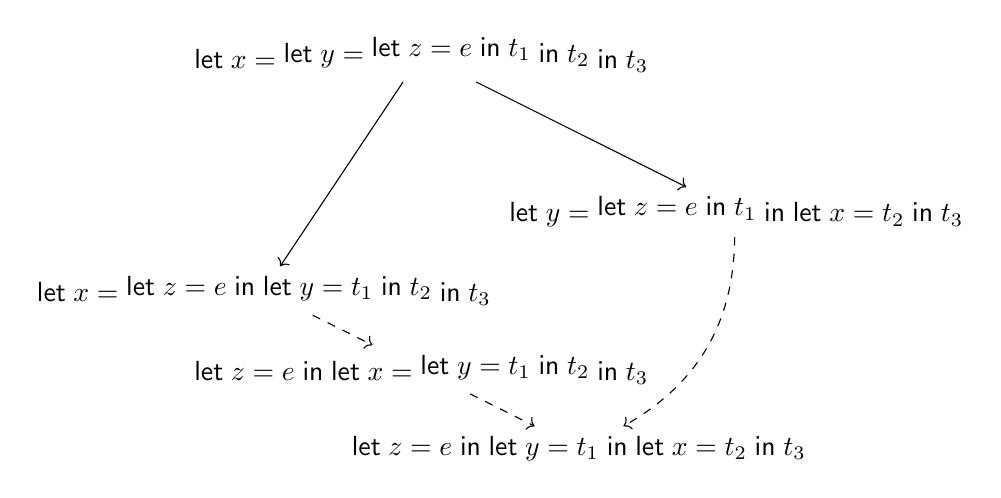
\begin{tikzpicture}
	\node (E1) at (2,5) {$\RLet{x}{\RLet{y}{\Let{z}{e}{t_1}}{t_2}}{t_3}$};
	\node (E2) at (6,3) {$\RLet{y}{\Let{z}{e}{t_1}}{\Let{x}{t_2}{t_3}}$};
	\node (E3) at (0,2) {$\RLet{x}{\Let{z}{e}{\Let{y}{t_1}{t_2}}}{t_3}$};
	\node (E3') at (2,1) {$\Let{z}{e}{\RLet{x}{\Let{y}{t_1}{t_2}}}{t_3}$};
	\node (E4) at (4,0) {$\Let{z}{e}{\Let{y}{t_1}{\Let{x}{t_2}{t_3}}}$};
	\path[->]
		(E1) edge (E2)
		(E1) edge (E3);
	\path[->,dashed]
		(E2) edge[bend left] (E4)
		(E3) edge (E3')
		(E3') edge (E4);
	%\draw [brown] (current bounding box.south west) rectangle (current bounding box.north east);
\end{tikzpicture}
$$
Two steps are needed on the left to complete the diagram.
This calls for the following generalization, which can do it in one step and \textit{does} have the diamond property:
$$\Let{x}{L[t_1]}{t_2} → L[\Let{x}{t_1}{t_2}]$$
However, this is not enough for \textit{parallel} reduction.
Here, the redex above overlaps with two different redexes below:
$$
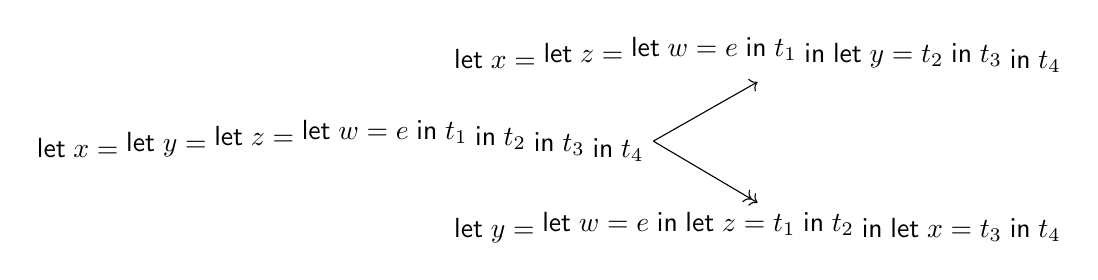
\begin{tikzpicture}
	\node (E1) at (0,0) {$\RLet{x}{\RLet{y}{\RLet{z}{\Let{w}{e}{t_1}}{t_2}}{t_3}}{t_4}$};
	\node (E2) at (5.3,1.1) {$\RLet{x}{\RLet{z}{\Let{w}{e}{t_1}}{\Let{y}{t_2}}{t_3}}{t_4}$};
	\node (E3) at (5.3,-1.1) {$\RLet{y}{\Let{w}{e}{\Let{z}{t_1}}{t_2}}{\Let{x}{t_3}}{t_4}$};
	\path[->] (E1.east) edge[] (E2.south);
	\path[->>] (E1.east) edge[] (E3.north);
	%\draw [brown] (current bounding box.south west) rectangle (current bounding box.north east);
\end{tikzpicture}
$$
To complete this diagram in one parallel reduction step, it would need to have not only length-wise, but also a depth-wise generalization
of $\KwLet$ reassociation.
We don't provide a definition here, since we haven't managed to prove any attempt right.

The other challenge is that a $let.\S$ reduction can tear apart a $let.let$ redex:
$$
\begin{tikzpicture}
	\node (E1) at (0,0) {$\Let{x}{\Let{y}{\S κ.\,e}{t_1}}{t_2}$};
	\node (E2) at (3.5,-2) {$\Let{y}{\S κ.\,e}{\Let{x}{t_1}{t_2}}$};
	\node (E3) at (-3.5,-1.333) {$\Let{x}{\S κ.\,e\subst{κ}{κ[\Let{y}{□}{t_1}]}}{t_2}$};
	\node (E3') at (-3.5,-2.666) {$\S κ.\,e\subst{κ}{κ[\Let{x}{\Let{y}{□}{t_1}}{t_2}]}$};
	\node (E4) at (0,-4) {$\S κ.\,e\subst{κ}{κ[\Let{y}{□}{\Let{x}{t_1}{t_2}}]}$};
	\path[->] (E1) edge (E2);
	\path[->] (E1) edge (E3);
	\path[->,dashed] (E3) edge (E3') (E2) edge (E4);
	\path[->>,dashed] (E3') edge (E4);
\end{tikzpicture}
$$
We need a successive $let.\S$ step to make the $let.let$ redexes whole, now after structural substitution.

\section{Conditional result}


\chapter{Adequacy}

\begin{theorem}[Strong postponement]
	$${\Rrightarrow · ↦} ⊆ {↦^* · \Rrightarrow}$$
\end{theorem}
\begin{proof}
	By induction on $\Rrightarrow$ and cases.
\end{proof}
\begin{corollary}
	${\Rrightarrow · ↦^*} ⊆ {↦^* · \Rrightarrow}$
\end{corollary}
\begin{proof}
	Induction on the length of $↦^*$.
\end{proof}

\begin{theorem}[Quasi-subcommutation of internal reduction and evaluation step]
 \label{quasisubcomm} 
	$${\Lleftarrow · ↦ } ⊆ {↦^= · \Lleftarrow · \mapsfrom^*}$$
\end{theorem}
\begin{proof}
	By induction on $\Lleftarrow$ and cases.
\end{proof}
\begin{corollary}[Subcommutation of standard reduction and evaluation step] \item
	${(\Lleftarrow · \mapsfrom^*) · ↦} ⊆ {↦^= \mathbin{·} ({{\Lleftarrow} · \mapsfrom^*})}$
\end{corollary}
\begin{proof}
	From the theorem % ${\Lleftarrow · ↦ } ⊆ {↦^= · \Lleftarrow · \mapsfrom^*}$
	and
	${(\Lleftarrow · \mapsfrom^+) · ↦} ⊆ {{{\Lleftarrow} · \mapsfrom^*}}$ (by determinism of $↦$)
\end{proof}
\begin{corollary}
	${(\Lleftarrow · \mapsfrom^*) · ↦^*} ⊆ {↦^* \mathbin{·} ({{\Lleftarrow} · \mapsfrom^*})}$
\end{corollary}
\begin{proof}
	Induction on the length of $↦^*$.
\end{proof}



%\begin{theorem}[Standardization]
%\end{theorem}
%\begin{corollary} \label{stanv}%
%	If $e →^* v$, then $e ↦^* v' →_i^* v$.
%\end{corollary}
%\begin{proof}
%	By standardization and since $→_i$ can't turn a nonvalue into a value.
%\end{proof}
\begin{lemma}
	${→} ⊆ {↦ ∪ \Rrightarrow}$
\end{lemma}

\begin{theorem}[Adequacy]
	If $e → e'$, then $e$ evals to a value iff $e'$ evals to a value.
\end{theorem}
\begin{proof}

%%	We take the proof from Crary.
%	If $e' ↦^* v$, then $e →^* v$. By corollary \ref{stanv} we have $e ↦^* v' →_i^* v$.
%
%	If $e ↦^* v$, then by confluence we have $v →^* v' ←^* e'$, where $v'$ must be a value
%	because $→$ preserves valueness. By corollary \ref{stanv} we have $e' ↦^* v'' →_i^* v'$.
	The case $e ↦ e'$ is easy, we consider $e \Rrightarrow e'$.

	\begin{enumerate}
		\item
			Assume $e ↦ e_1 ↦ ... ↦ e_n = v$.
			We prove $e'$ evals to a value by induction on $n$.

			If $e=e_n=v$, then $e'$ is a value since $\Rrightarrow$ preserves valueness.

			Otherwise, apply subcommutation for $e' \Lleftarrow e ↦ e_1$.
			We obtain $e' ↦^? e'_1 \Lleftarrow · \mapsfrom^* e_1$ for some $e'_1$.
			Since evaluation steps are deterministic and not possible beyond $e_n$,
			we have $e_i \Rrightarrow e'_1$ for some $i$ s.t.\,$1 ≤ i ≤ n$.
			By induction for $e'_1 \Lleftarrow e_i ↦^* v$ we get $e'_1 ↦^* v'$ for some value $v'$.
			Therefore $e' ↦ e'_1 ↦^* v'$.

		\item
			Assume $e' ↦ e'_1 ↦ ... ↦ e'_n = v$.
			We prove $e$ evals to a value by induction on $n$.

			If $e'=e'_n=v$, then $e$ is a value since $\Rrightarrow$ can't make a nonvalue a value.

			Otherwise, apply postponement for $e \Rrightarrow e' ↦ e'_1$.
			We obtain $e ↦^* e'' \Rrightarrow e'_1$ for some $e''$.
			By induction for $e'' \Rrightarrow e'_1 ↦^* v$ we know that $e''$ evals to a value,
			so $e$ also does.

	\end{enumerate}
\end{proof}

%In the above, instead of confluence ${←^* · →^*} ⊆ {→^* · ←^*}$ we could have used
%commutation ${← · ↦^*} ⊆ {↦^* · ←^*}$.
%This could be easier to prove, but we do not explore this approach in this work.

\begin{corollary}[Contextual equivalence, observing termination to a value]
	\label{ctxeqv1}
	If $e → e'$, then for all general contexts $C$, $C[e]$ evals to a value iff $C[e']$ evals to a value.%
\end{corollary}
\begin{proof}
	By congruence of reduction and adequacy.
\end{proof}

The above notion of contextual equivalence isn't the most common one.
But we can deduce the usual notion from it using the argument of \cite{bisim}.

\begin{prop}[Stuck terms]
\end{prop}

\begin{theorem}[Contextual equivalence, observing termination]
	If $e → e'$, then for all closing contexts $C$, $C[e]$ terminates iff $C[e']$ terminates.
\end{theorem}
\begin{proof}
	By \ref{ctxeqv1} it suffices to show that
	$C[e]$ terminates to a nonvalue iff $C[e']$ terminates to a nonvalue.
\end{proof}

\chapter{Abella mechanization}

\chapter{Related work}


\section{Distributing delimiters}
There is a strand of work which tackles static delimited control from the opposite direction.
Whereas we use structural reduction so that S moves closer to the delimiter, that strand's defining feature is
the delimiter distributing over let expressions so that \textit{a} delimiter can meet the control operator:

There, the return clause is an integral part of the syntax. On a sequence of lets this becomes

We consider turning every let into a delimiter unsatisfactory, since delimiters usually have a much higher runtime cost than let bindings.

Because they lack structural reduction, those systems cannot perform the optimizations in examples TODO.
We show that translations from those calculi preserve equations (understood as the equivalence closure of reduction)
to argue that our calculus is more powerful.

\section{shift0 calculus}
By reflection\cite{ppdp21} it follows that the original shift0 equational theory by Materzok is also less powerful,
but for completeness we show it directly.

\section{Delimited \texorpdfstring{$λμ$}{lambda-mu}}

\section{Expressing handlers using shift0}

\section{Fine-grained syntax for algebraic operations}
The original syntax for algebraic operations involved continuations.
What we may now express as the generic effect $arb : Bool$
can be equivalently expresssed as an algebraic operation $or : (unit → τ)^2 → τ$
with the equivalences $arb = or(λ\_.\,true, λ\_.\,false)$ and
$or(k_1,k_2) = if arb then k_1 () else k_2 ()$ \cite{alggen}.

%Handling of algebraic operations can be characterized by equalities \cite{handlers}, viz.
%$$\Handle \Op(x_1.\,t_1,...,x_n.\,t_n) \With k_1,...,k_n.\,t_h =$$

The connection of algebraic operations and control wasn't explicitly noted at first,
but can be seen in the naturality condition for algebraic operations,
which states that evaluation contexts commute with operations \cite{logic, handling}:
$$E[\Op(x_1.\,t_1, ..., x_n.\,t_n)] = \Op(x_1.\,E[t_1], ..., x_n.\,E[t_n])$$

The calculus in \cite{hia} has an intermediate approach,
where an operation has only one continuation parameter.
The intended surface syntax is of the generic effect form $\Op v$,
which is elaborated to start with an identity continuation $\Op v\,(λx.\,x)$.
The step relation captures the evaluation context in a fine-grained manner:
$$\Let{y}{\Op v\,(λx.\,t_1)}{t_2} ↦ \Op v\,(λx.\,\Let{y}{t_1}{t_2})$$
This bears similarity to our approach based on structural reduction.
However, we don't see a way to express our optimizations without introducing $\abort$ in some form.

\section{Confluence}

Proofs of confluence have been notoriously difficult since the beginning --
the many early attempts for the $λ$-calculus were flawed.

The proof alongside the introduction of the $λμ$-calculus \cite{parigot92} also turned out to be incorrect \cite{baba}.
The fix involves performing multiple structural reduction steps \cite{baba,koji}, which we have employed in our formalization
and verified that it works also with our tail-of-delimiter reductions.

Herbelin and Zimmerman \cite{Herbelin} claim that a proof by parallel reduction is possible for a $λμ$-calculus with
$\KwLet$ reassociation, but provide no details. We don't see how they could deal with the $let.\S$-$let.let$ critical pair
unless they add a $κ[\Let{x}{e}{t}] → \Let{x}{e}{κ[t]}$ reduction, which is similar to theirs
$x(\Let{x}{e}{t}) → \Let{x}{e}{xt}$ and seems to be valid in the undelimited setting.

The proof in \cite{ppdp21} is claimed by local confluence of $\Rightarrow$ such that $→^*=\Rightarrow^*$,
which is not a valid argument (take $\Rightarrow=→$ for a counterexample, it is known that local confluence does not imply confluence). Diamond property is needed instead of local confluence.



\section{Tail reductions and letcc}
The central idea in our paper is the reduction
$$⟨L[\S κ.\,e]⟩ → ⟨L[\A\,e\subst{κ}{⟨□⟩}]⟩$$
It is tempting to decompose $\S$ into its constituent parts:
a $\keyword{letcc}$ which binds the continuation without aborting, and an abort $\A$:
$$\S κ.\,e ≡ \keyword{letcc}\;κ.\,\A\,e$$
Then we could simulate $dL.\S$ using a reduction that pushes $\keyword{letcc}$ out of the tail:
$$\Let{x}{e}{\keyword{letcc}\;κ.\,t} → \keyword{letcc}\;κ.\,\Let{x}{e}{t}$$
Analogous reductions have been considered for undelimited continuations.

There are issues with this approach, though:
\begin{enumerate}

	\item
Because $\keyword{letcc}$ binds the continuation and keeps running in it
$$⟨E[\keyword{letcc}\;κ.\,e]⟩ ↦ ⟨E[e\subst{κ}{⟨E⟩}]⟩$$
it seems inherently incompatible with one-shot (linear) continuations.
This is a design choice or a limitation of some implementations of control, e.g.\,OCaml 5.
\item

The above reduction isn't semantics-preserving. If $e$ above is the nonterminating $Ω$,
then the left side diverges, while the right side gets stuck on searching for a delimiter.
We could ensure a delimiter is found by performing the reduction only in $⟨L⟩$,
but then it is unclear if there are serious benefits to this approach.
\end{enumerate}


\section{Expressing return clauses}
Recall our encoding of return clauses:
$$⟨e│x.\,e_r⟩ ≡ ⟨\Let{x}{e}{\A\;e_r}⟩$$
$$\Handle e \With x,k.\,e_h │ x.\,e_r ≡ ⟨\Let{x}{e}{\A\;e_r}│λx,k.\,e_h⟩$$
An equivalence reminiscent of it has been proven for typed algebraic effects \cite{hwc}:
$$\Handle e \With x,k.\,e_h │ x.\,e_r ≈\Handle \Let{x}{e}{\Lift{e_r}} \With x,k.\,e_h$$
After $e$ has finished evaluating and we start evaluating the rhs of $\KwLet$,
we know that the frame at the top of the stack will be the handler.
So instead of adding a $\KwLift$ stack frame that makes effects skip the $\KwLift$-handler pair \cite[Appendix A]{hwc},
we can just pop the handler with an $\A$ for an equivalent result.
Our approach is therefore slightly more space- and time-efficient.

\chapter{Discussion and future work}

While this work brings forth many new ideas, it is far from being the IR of a compiler.

We believe all results transfer to multi-prompt delimited control, where we have independent sets of labeled operators $S^\ell κ. e$, $⟨e⟩^\ell$.
This is necessary for working with multiple effects, though the lift construct can to some extent simulate that.
Naturally, the purity assertions also could be refined to block or allow specific listed effects.
The multi-prompt calculus need a mild form of typing: in the renaming reduction we need to know that the continuation variable $κ$ comes
from an $\S$ with the matching label
$$κ^\ell[\S^\ell κ'.\,e] → e\subst{κ'}{κ}$$

One could wonder why we don't have tail-of-plug reductions
$$κ[L[\S κ'.\,e]] → κ[L[A\,e\subst{κ'}{κ}]]$$
The reason is they don't work in the multi-prompt setting.
If $κ$ is allowed to have delimiters of different labels in the middle, then
the continuation may not be intact by the time we get to the $\S$.

It should be clear that the central idea of this work, the tail-of-delimiter reductions,
doesn't apply to \textit{dynamic} delimited control.
They are those that make the delimiter disappear after capture, for example \textsf{control\textsubscript{0}}:
$$⟨E[\mathsf{control_0} κ.\,e]⟩ ↦ e\subst{κ}{E}$$
The only hope for optimizations seems to be purity-aware reductions,
which could move the delimiter directly to the operator. The same applies to the related \textit{shallow} effect handlers.
There is however an option between shallow and deep handlers: \textit{sheep} handlers \cite{sheep},
where the delimiter is static,
but the dynamically bound interpretation of the effect can be used at most once
and has to be manually reinstated every time a continuation is installed.




Realistic languages also have more tail contexts such as $if b then □ else □$ as well as evaluation contexts.

join points?

%\hfuzz=1pt
\printbibliography[heading=bibintoc]

\end{document}
